% Native syntax: tikzlibrarydecorations.softclip.code.tex:405-430 (path key).
% The upper cubic enters at the left face x=0.7 and exits at the top face
% y=2.05, away from any corner. PGF splits at both times on the original
% cubic in one operation; successive x-only and y-only clips differ.
% The horizontal red path meets only the left face. Source strokes stay whole.
\documentclass[border=2pt]{standalone}
\usepackage{pgfplots}
\usepgfplotslibrary{fillbetween}
\pgfplotsset{compat=1.18}
\begin{document}
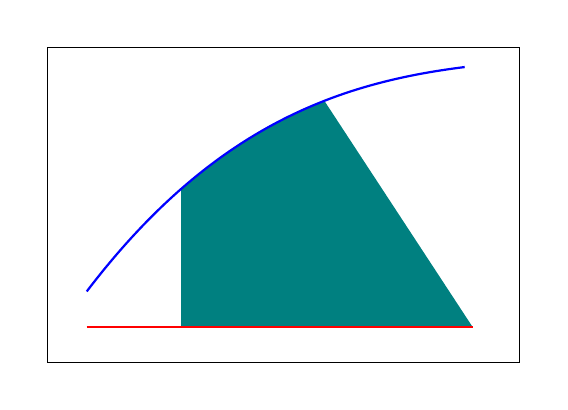
\begin{tikzpicture}
  \begin{axis}[at={(0,0)},anchor=south west,width=6cm,height=4cm,scale only axis,
    xmin=-1,xmax=5,ymin=-1,ymax=3,enlargelimits=false,axis lines=box,ticks=none]
    \draw[blue,thick,name path=rise] (axis cs:-0.5,-0.1)
      .. controls (axis cs:1.1,2) and (axis cs:2.7,2.55) .. (axis cs:4.3,2.75);
    \addplot[red,thick,mark=none,name path=datum] coordinates {(-0.5,-0.55) (4.4,-0.55)};
    \addplot[draw=none,fill=teal] fill between[of=rise and datum,
      soft clip={path={(axis cs:0.7,-0.8) rectangle (axis cs:4.7,2.05)}}];
  \end{axis}
  \path[use as bounding box] (-0.25,-0.25) rectangle (6.25,4.25);
\end{tikzpicture}
\end{document}
